\section{Analyse des performances}











 
%%%%%%%%%%%%%%%%%%%%%%%%%%%%%%%%%%%%%%%%%%%%%%%%%%%%%%%%%%%%%%%%%%%%%%%%%%%%%%%%%%%%%%%%%%%%%%%%%%%%%%%%%%%%%%%%%%%%%%%%%%%%%%%%%%%%%%%%%%%%%%%%%%%%%%%%%%%%%%%%%%%%%%%%%%%%%%%%%%%%%%%%%%%%%%%%%%%%%%%%%
\subsection{Analyse de performances}%%%%%%%%%%%%%%%%%%%%%%%%%%%%%%%%%%%%%%%%%%%%%%%%%%%%%%%%%%%%%%%%%%%%%%%%%%%%%%%%%%%%%%%%%%%%%%%%%%%%%%%%%%%%%%%%%%%%%%%%%%%%%%%%%%%%%%%%%%%%%%%%%%%%%%%%%%%%%%%%%%%%%%%%%%%%%%%%%%%%%%%%%%%%%%%%%%%%%%%%%



%%%%%%%%%%%%%%%%%%%%%%%%%%%%%%%%%%%%%%%%%%%%%%%%%%%%%%%%%%%%%%%%%%%%%%%%%%%%%%%%%%%%%%%%
%%% |   _  \      /  __  \   /  __  \  |   ____|   |  |     |  | |  \ |  | |   ____| %%%
%%% |  |_)  |    |  |  |  | |  |  |  | |  |__      |  |     |  | |   \|  | |  |__    %%%
%%% |      /     |  |  |  | |  |  |  | |   __|     |  |     |  | |  . `  | |   __|   %%%
%%% |  |\  \----.|  `--'  | |  `--'  | |  |        |  `----.|  | |  |\   | |  |____  %%%
%%% | _| `._____| \______/   \______/  |__|        |_______||__| |__| \__| |_______| %%%
%%%%%%%%%%%%%%%%%%%%%%%%%%%%%%%%%%%%%%%%%%%%%%%%%%%%%%%%%%%%%%%%%%%%%%%%%%%%%%%%%%%%%%%%

\subsubsection{Modèle du Roofine} \label{sec:roofline}
%%%%%%%%%%%%%%%%%%%%%%%%%%%%%%%%%%%%%%%%%%%%%%%%%%%%%%%%%%%%%%%%%%%

%%%%%%%%%%%%%%%%%
\paragraph{Motivation et objectifs}
%%%%%%%%%%%%%%%%%
Présenté par William et al. en 2009 \cite{Williams2008}, le modèle du \textit{roofine} est un modèle de performance simple qui représente graphiquement les performances d’un code en situant sa performance par rapport au performances maximales de l’architecture. L’objectif principale de ce modèle est de donner le pourcentage de la performance disponible atteinte par un code. L’intérêt de ce model est de restreindre l’analyse de performance aux deux ressources importantes pour les applications HPC: la performance calculatoire (GFLOP/s) et la performance du bus mémoire (GB/s).
Le modèle est utilisé pour représenter les différentes fonctions clefs d’une application. Ainsi, le programmeur pourra commencer son travail d’optimisation sur les fonctions avec le plus de potentiel.

\begin{figure}
    \center
    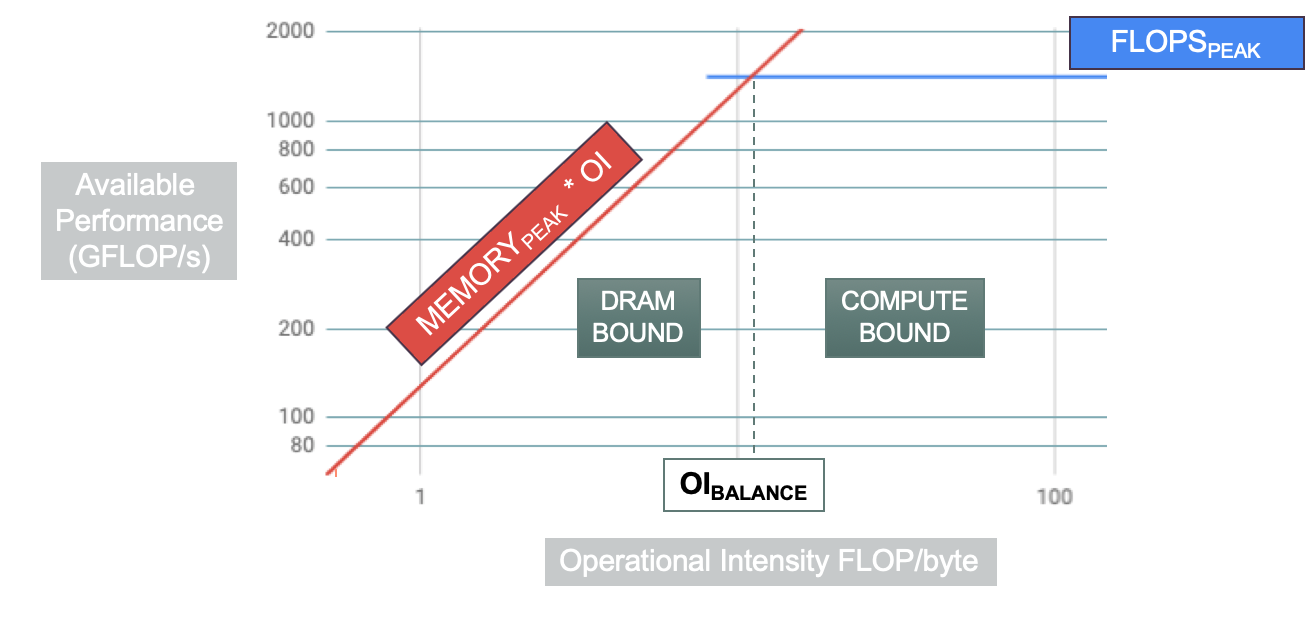
\includegraphics[width=10cm]{images/roofline.png}
    \caption{\label{fig:roofline} Représentation graphique du modèle du \textit{roofline}. En fonction de son l'intensité opérationnelle, la performance d'un code sera limitée par la bande passante ou par le processeur.}
\end{figure}


La \autoref{fig:roofline} montre une représentation du modèle du \textit{roofine}. Sur l’axe des abscisse est représentée l’intensité opérationnelle de l’algorithme (en flops/byte) qui correspond nombre d’opération flottante appliqué à chaque byte de donnée amené depuis la mémoire. Sur l’axe des ordonnées est représentée la performance de calcul mesurée en GFLOP/s.
Chaque hot spot sont placés en fonction de leur intensité opérationnelle, calculée à partir de la lecture du code, et de sa performance, mesurée lors de l’exécution.

%%%%%%%%%%%%%%%%%
\paragraph{Preuve et construction}
%%%%%%%%%%%%%%%%%
L’objectif du modèle est de déterminer si la performance du code pour une architecture donnée est structurellement limité par la performance du processeur ($FLOPS_{peak}$ en $GFLOP/s$) ou bien par la performance du bus mémoire ($MEMORY_{peak}$ en $GB/s$). Une application réalisant la lecture de deux nombres pour y réaliser des centaines d’opérations verra ses performances limitées par la capacité de calcul $FLOPS_{peak}$ du processeur. Inversement, une application devant lire un grand jeu de données pour ne réaliser qu'une opération sur chaque valeur, verra ses performance limitées par celle du bus mémoire $MEMORY_{peak}$. On peut estimer la quantité de calculs à réaliser sur chaque donnée en calculant son Intensité Opérationnelle  ($\text{OI}$ en $flop/byte$). Pour cela il faut lire le code source pour compter manuellement le nombre d’opérations réalisées ($\text{\#FLOP}$) et le nombre de données nécessaires chargées depuis la mémoire ($\text{\#BYTE}$). On peut ainsi calculer l’Intensité Opérationnelle d’un code en faisant le ratio des deux valeurs.

\begin{equation}
\begin{aligned}
        \text{OI}_{kernel} =\ &\cfrac{\text{\#FLOP}}{\text{\#BYTE}}
\end{aligned}
\end{equation}

Le temps pour exécuter le code ($\text{TEMPS}_{theorique}$), sera le temps mis par la ressource la plus utilisée par le code. On peut estimer ce temps par la formule suivante.
\begin{equation}
\begin{aligned}
     \text{TEMPS}_{theorique} =\  &max 
     \begin{cases} 
        \quad \cfrac{\text{\#FLOP}}{\text{FLOPS}_{peak}}    \\[15pt]
        \quad \cfrac{\text{\#BYTE}}{\text{MEMORY}_{peak}}
    \end{cases}
\end{aligned}
\end{equation}




La performance théorique du code ($\text{PERF}_{theorique}$ en GFLOP/s) peut être calculée grâce aux transformations successives de l'\autoref{eq:PERFT}.
\begin{equation}
\begin{aligned}
\label{eq:PERFT}
\cfrac{\text{TEMPS}_{theorique}}{\text{\#FLOP}}  =\ &\text{max}
\begin{cases} 
    \cfrac {1}{\text{FLOPS\_{peak}}}    \\[15pt]  
    \cfrac {\cfrac{\text{\#BYTE}}{\text{MEMORY}_{peak}}}{\text{\#FLOP}} 
\end{cases}\\[20pt]
\cfrac{\text{\#FLOP}}{\text{TEMPS}_{theorique}}  =\ &\text{min}
\begin{cases} 
    \text{FLOPS}_{peak}    \\[15pt]  
    \cfrac{\text{\#FLOP}}{\text{\#BYTE}} \times \text{MEMORY}_{peak}
\end{cases}\\[20pt]
\text{PERF}_{theorique}  =\ &\text{min}
\begin{cases} 
    \text{FLOPS}_{peak}    \\[15pt]  
    \text{OI}_{kernel} \times \text{MEMORY}_{peak} 
\end{cases}
\end{aligned}
\end{equation}



Pour une architecture, il faut déterminer pour quelle intensité opérationnelle une application est limitée par la mémoire ou le processeur. Pour cela, il faut calculer l’intensité opérationnelle ($\text{OI}_{balance}$) correspondant au croisement des deux droites sur la \autoref{fig:roofline}. 

\begin{equation}
\begin{aligned}
 \text{FLOPS}_{peak} =\ &\text{OI}_{balance} \times \text{MEMORY}_{peak} \\[20pt]
 \text{OI}_{balance} =\ &\frac{\text{MEMORY}_{peak}} {\text{FLOPS}_{peak}} 
\end{aligned}
\end{equation}

Une application dont l’intensité opérationnelle est inférieure à $\text{OI}_{balance}$ verra sa performance limitée par le système mémoire. Plus rarement, si l’intensité opérationnelle d’une application est supérieure à $\text{OI}_{balance}$, la performance sera alors limitée par le processeur.

\paragraph{Construction}
La première étape dans la construction du graphique est de tracer les deux axes limitant les performances d’un code. Ces deux droites représentes les performances crêtes de la mémoire et du processeur. Pour obtenir ces valeurs, elles peuvent être calculées à partir des spécifications du processeurs. Cependant, avec la complexification des architectures, il est difficile de les atteindre même avec des benchmarks prévus à cet effet. Il est donc préférable de les représenter par des valeurs mesurées comme indiqué dans la littérature  \cite{farjallah2014preparing}. Pour la mémoire le benchmark Stream peut être utilisé. Pour la performance du processeur, nous utilisons le générateur de benchmark présenté dans la \autoref{sec:kg}. D’autres travaux sont venus compléter les benchmarks disponibles pour caractériser l’architecture \cite{lo2014roofline}.




%%%%%%%%%%%%%%%%%
\paragraph{Évolutions}
%%%%%%%%%%%%%%%%%


Le \textit{roofine} a reçu de nombreuse améliorations depuis sa création. En 2014, les travaux \cite{Ilic2014} constate que le modèle originale n’est pas suffisament précis à cause de la faible précision de caractérisation de l’architecture. En effet, un code pouvant profiter de la localité des données dans les caches pourrait atteindre des performances supérieur au maximum prévu par le modèle utilisant seulement le bande passante mémoire. Inversement, la performance crête est calculé pour un code utilisant tous les coeurs du processeur, avec des instructions FMA vectorisées. Cependant, par leur nature, certain code ne peuvent pas utiliser ces  caractéristiques. La performance crête étant alors impossible à atteindre. Le modèle Cache-Aware Roofline Model (CARM) \cite{Ilic2014} a ainsi été développé permettant de représenter la performance des différents niveaux de caches. Cependant, le programmeur doit comprendre si son application peut tirer partie de cette localité, ce qui peut rendre cette approche plus difficile. Le modèle à depuis été affiné avec le Locality Aware Roofline Model (LARM) \cite{Denoyelle2018} permettant de modéliser les accès en mémoire non uniforme (NUMA).
D’autres travaux essaient d’automatiser sa construction \cite{lo2014roofline} pour faciliter son usage. L’outil de profiling d’Intel a intégré les modèles CARM et LARM pour automatiser la recherche des hot spot et afficher leur performance sur un même graphique. Pour cela, il désassemble le code et calcule l’intensité opérationnelle de la boucle étudiée.


%%%%%%%%%%%%%%%%%
\paragraph{Critiques}
%%%%%%%%%%%%%%%%%

La force de cette approche est de montrer rapidement au programmeur si son application est efficace ou non. Dans le cas échéant, il sait s’il doit travailler sur l’optimisation des flops ou de la mémoire. En modélisant les principaux kernels de son application, le programmeur saura sur lesquels ses optimisations seront le plus bénéfiques.

Bien d’ayant reçu de nombreuses améliorations, ce modèle doit être utilisé pour commencer l’analyse de performance. Mais il ne permet pas de modéliser n’y de comprendre finement la raison d’une performance.
La majorité des applications étant limitée par la bande passante mémoire, il est rare d’utiliser ce modèle pour modéliser la performances des unités de calculs. Mais il peut être intéressant de calculer l’intensité opérationnelle d’une boucle pour s’en assurer avant d’apporter des optimisations. De plus, les accélérateurs à venir essaient de réduire le trou de performance entre les processeurs et la mémoire. Cette modélisation est donc importante pour l’analyse de performance.
